\documentclass[12pt]{report} % Khuyên dùng 12pt chuẩn, hoặc dùng exttreport nếu bắt buộc 13pt
\usepackage[utf8]{inputenc}
\usepackage[T5]{fontenc}
\usepackage{tikz}
\usepackage{multirow}
\usepackage{geometry}
\usepackage{float}
\usepackage{lmodern}
\usepackage{graphicx}
\usepackage{subcaption}
\usepackage{xcolor}
\setlength{\parindent}{0pt}
\geometry{a4paper, margin=2.5cm}


\begin{document}

\begin{center}
    \large TRƯỜNG ĐẠI HỌC MỞ TP.HCM\\
    KHOA CÔNG NGHỆ THÔNG TIN\\[0.2em]
    \rule{0.4\textwidth}{0.4pt}\\[1cm]
    
    \LARGE\textbf{Phân tích các yếu tố và ứng dụng Học Máy dự đoán khả năng bệnh nhân tái nhập viện ở Mỹ}
\end{center}

\vspace{0.25cm}

\begin{center}
\textbf{Môn học:} Phân tích dữ liệu\\
\end{center}
\textbf{Giảng viên hướng dẫn:} Ph.D Hồ Hướng Thiên\\
\textbf{Thành viên:} Trần Thị Thanh Thảo\textsuperscript{Nhóm trưởng}, Bùi Công Thiệt



\section*{Tóm tắt}

Sức khỏe là một trong các yếu tố ảnh hưởng đến đời sống của con người, đặc biệt là tình trạng tái nhập viện cũng phản ánh được một phần sức khỏe của người dân.
Với bộ dữ liệu \ref{table:description_data} là dữ liệu tới tình trạng sức khỏe và tỉ lệ tái nhập viện của bệnh nhân. Từ đó, ứng dụng các thuật toán ML để dự đoán khả 
năng tái nhập viện bằng cách ứng dụng các thuật toán Logistic Regression, Random Forest, XGBoost, LightGBM và kết quả mang lại rất khá ổn với chỉ số Accuracy đạt 64.6\% và ROC-AUC đạt 70.9\%. Bên cạnh đó
vẫn còn một số hạn chế mà phải cần cải thiện, đặc biệt là bộ dữ liệu cần được cập nhật phù hợp với tình trạng ở các năm gần đây hơn, ngoài ra vẫn chưa ứng dụng được các mô hình tiên tiến để nâng cao hiệu năng và khai thác hết tiềm năng dữ liệu.

\section*{Giới thiệu}

Trong thời gian gần đây, việc tái nhập viện của bệnh nhân đã trở thành một
vấn đề quan trọng và được quan tâm trong lĩnh vực y tế. Tái nhập viện không chỉ
ảnh hưởng đến sức khỏe của bệnh nhân mà còn là một thách thức lớn đối với
hệ thống chăm sóc sức khỏe. Vì thế để góp phần giải quyết vấn đề này, việc
phân tích các yếu tố ảnh hưởng đến khả năng tái nhập viện của bệnh nhân
và dự đoán khả năng tái nhập viện.

\section*{Khám phá dữ liệu}
Về bộ dữ liệu, bộ dữ liệu được nghiên cứu và tổng hợp bởi nhóm tác giả John Clore và cộng sự. Bộ dữ liệu được tổng hợp của
130 bệnh viện ở Mỹ, với các chỉ số như race, gender,... với hơn 100.000 dòng dữ liệu.

Kiểm tra sự phân bổ của các thuộc tính cũng là một phần quan trọng để xác định tính chính xác của dữ liệu. Dữ liệu dạng số được thể hiện thông qua các hình \ref{fig:data_overview} và \ref{fig:matrix_corr}.

\begin{figure}[H]
    \centering
    \begin{subfigure}{0.48\textwidth}
        \centering
        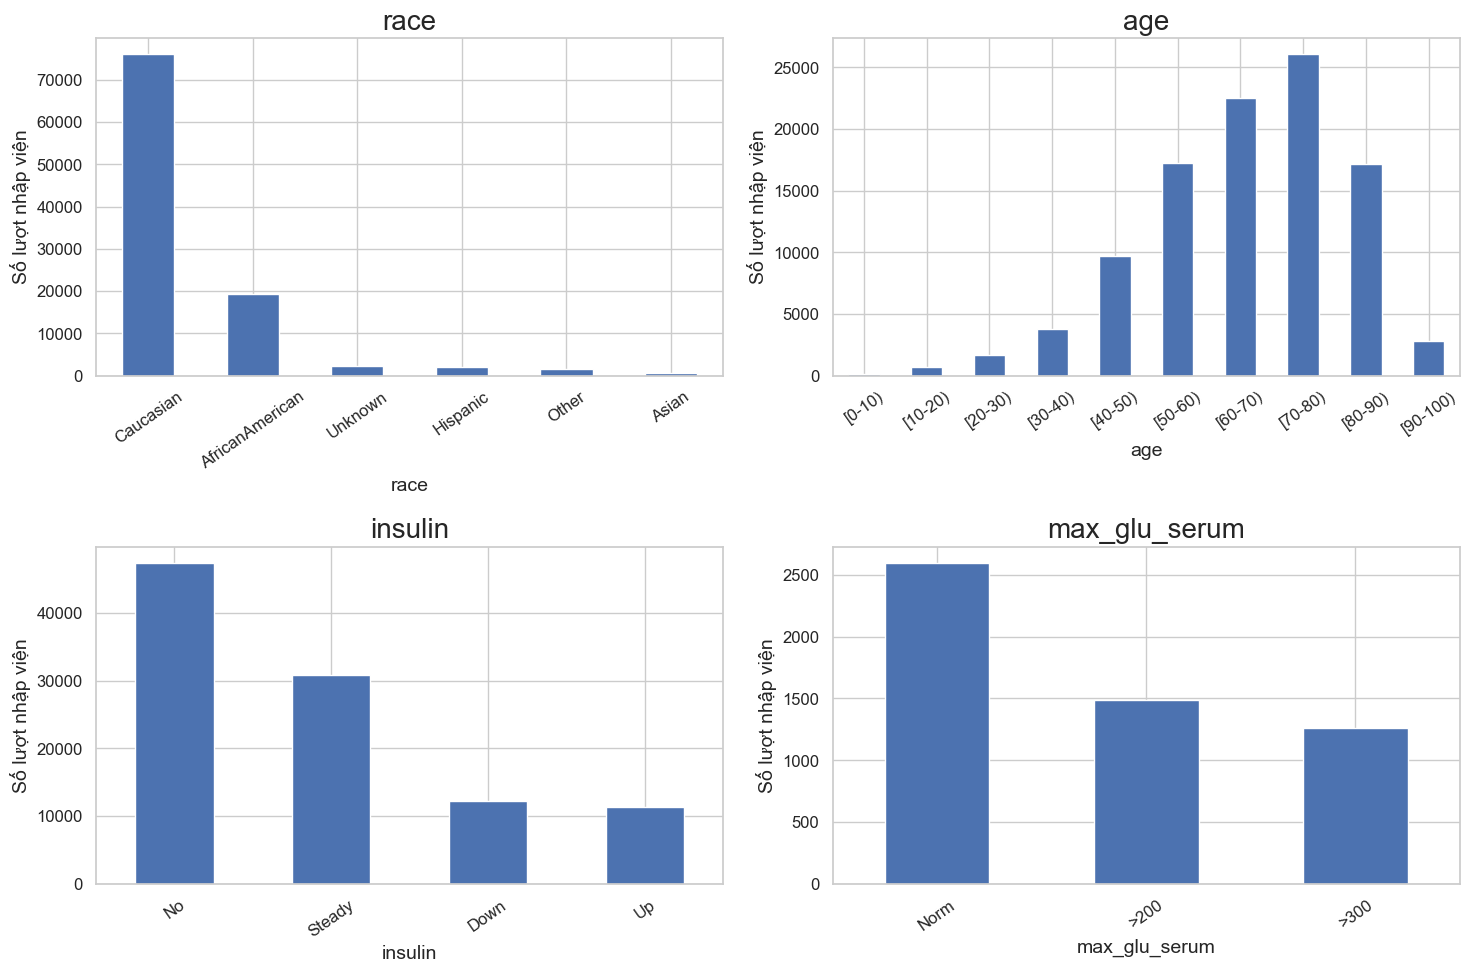
\includegraphics[width=\textwidth]{../asset/group1.png}
        \caption{Phân bổ của các thuộc tính số ở Nhóm 1}
        \label{fig:target}
    \end{subfigure}
    \hfill
    \begin{subfigure}{0.48\textwidth}
        \centering
        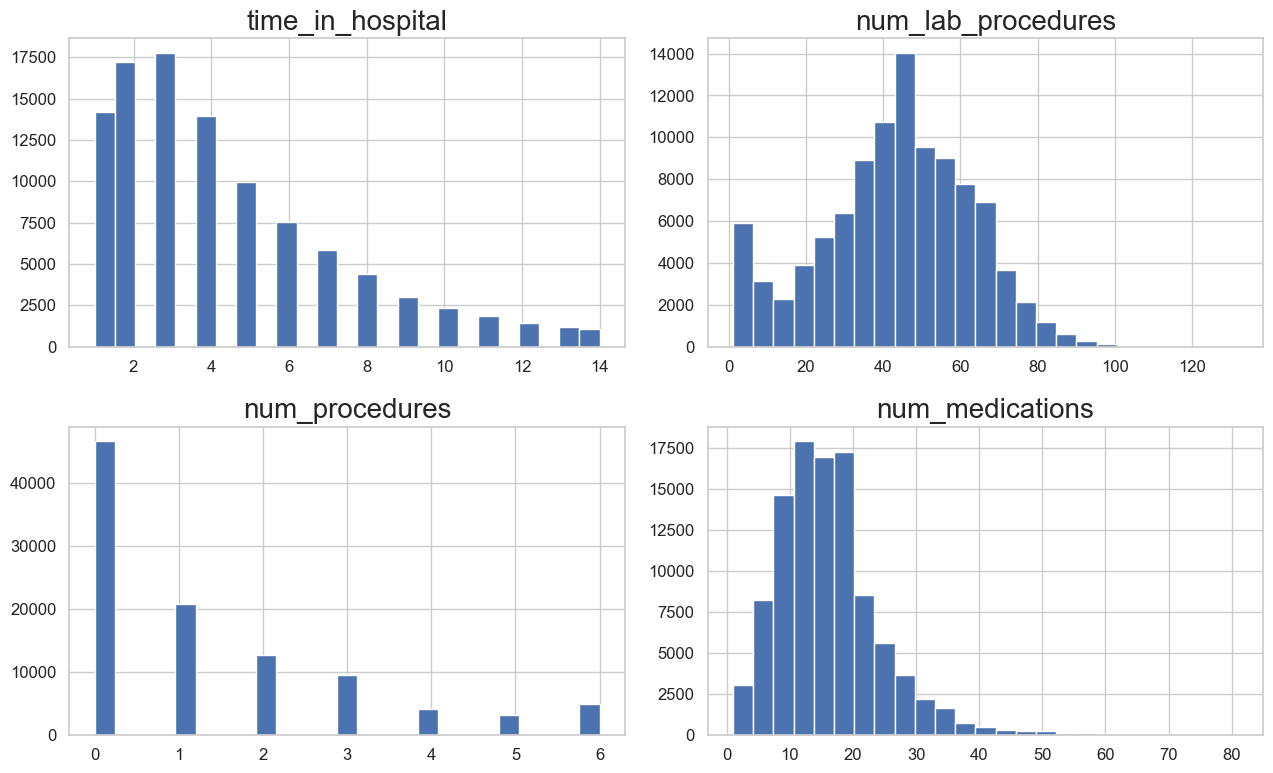
\includegraphics[width=\textwidth]{../asset/group2.png}
        \caption{Phân bổ của các thuộc tính số ở Nhóm 2}
        \label{fig:missing}
    \end{subfigure}

    \caption{Tổng quan dữ liệu}
    \label{fig:data_overview}
\end{figure}
\begin{figure}[H]
    \centering
    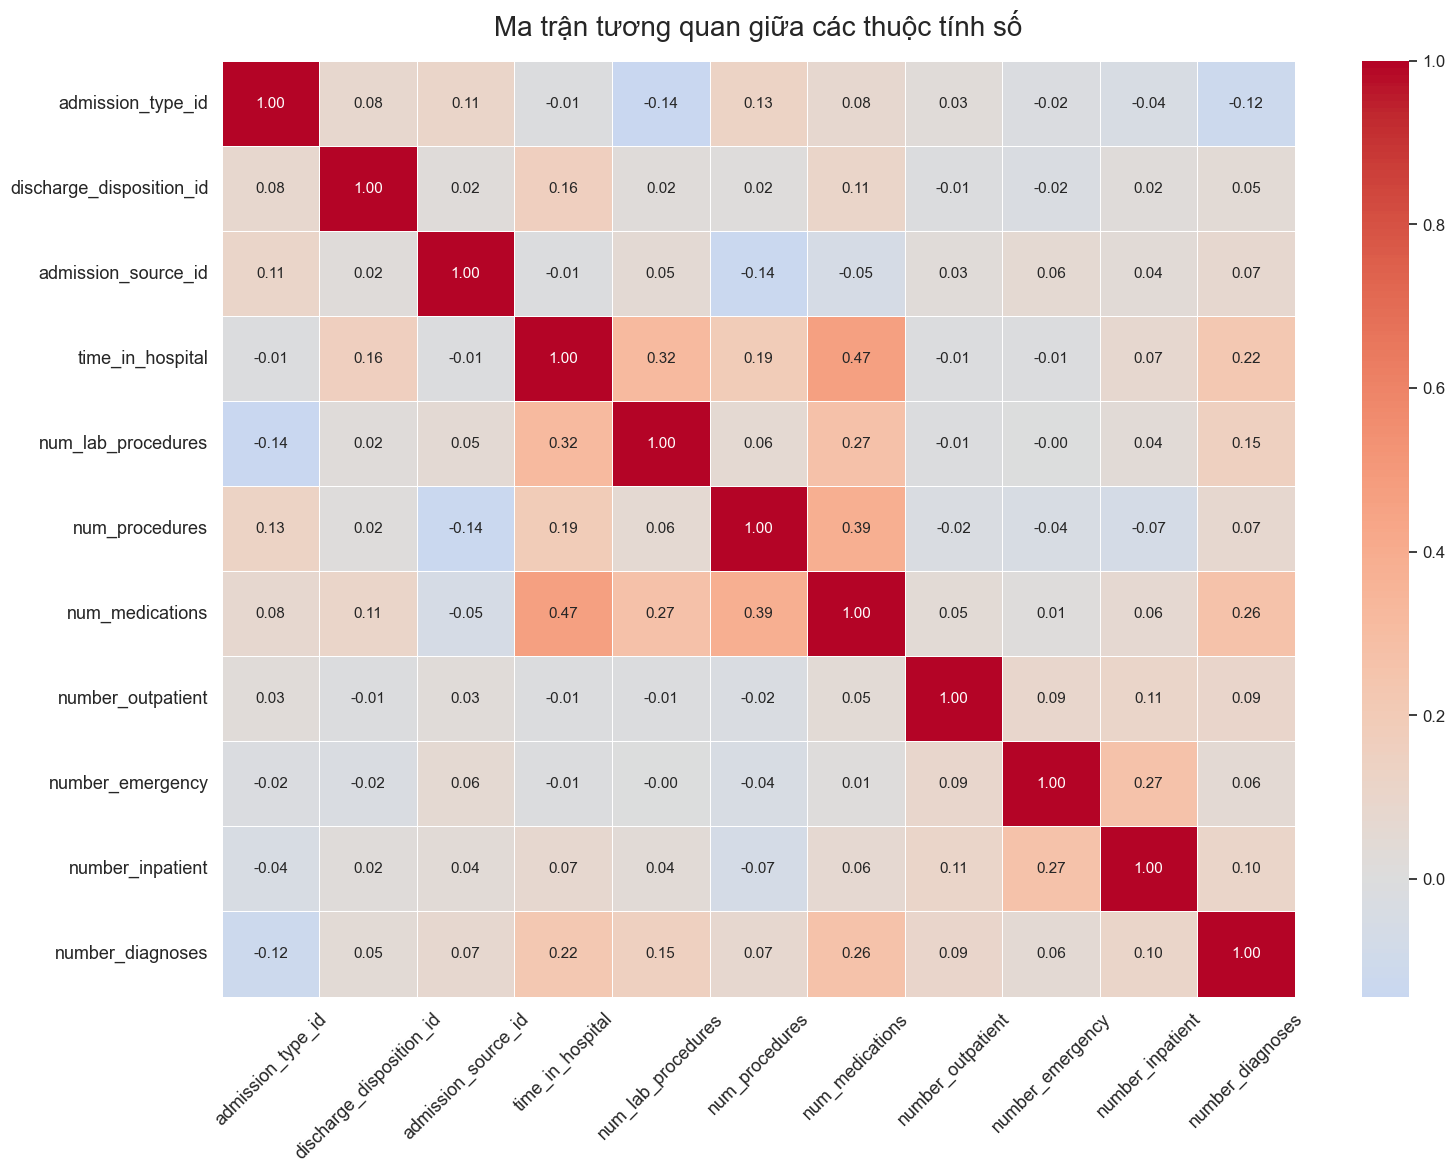
\includegraphics[width=0.6\textwidth]{../asset/matrix_corr.png}
    \caption{Ma trận tương quan giữa các thuộc tính}
    \label{fig:matrix_corr}
\end{figure}

Ngoài ra cũng có thể thấy rằng, mối tương quan rất lớn giữa \texttt{number\_inpatient} và \texttt{readmitted}. Từ đây cũng phản ánh một vấn đề thực tế rằng, một bệnh nhân nếu
họ nhiều lần nhập viện (không kể lý do) thì khả năng tái nhập viện của họ rất cao.

\begin{figure}[H]
    \centering
    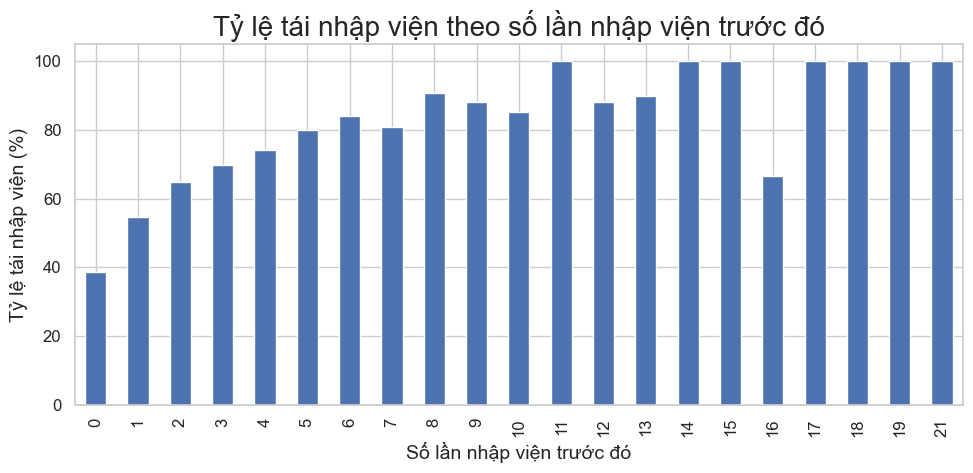
\includegraphics[width=0.6\textwidth]{../asset/inpatient.png}
    \caption{Mối tương quan giữa "inpatient" và "readmitted"}
\end{figure}

Và như được đề cập, vì bộ dữ liệu có hiện tượng bị mất mát dữ liệu và trong quá trình kiểm tra các dữ liệu bị missing được thay bằng
"?". Với dữ liệu với mục tiêu bao gồm các nhãn: ["No", "<30", ">30"], thì đây là bài toán phân loại đa lớp nhưng với số lượng nhãn hiện tại thì
rất khó để làm phân loại đa lớp, như hình sau \ref{fig:target_distribution}.

\section*{Phương pháp}

Để xử lý các giá trị missing, chuyển đổi các giá trị đang là "?" thành giá trị rỗng(NULL/None) để xử lý, ngoài ra các đặc trưng bị missing value nhiều như hình \ref{fig:missing_value} thì sẽ thực hiện bỏ thuộc tính đó để tránh gây ra tình trạng 
sai lệch dữ liệu.

Ứng dụng phương pháp "SelectKBest" để tìm ra các thuộc tính ảnh hưởng đến mô hình. Bên dưới là một số Feature được lựa chọn:

\begin{figure}[H]
    \centering
    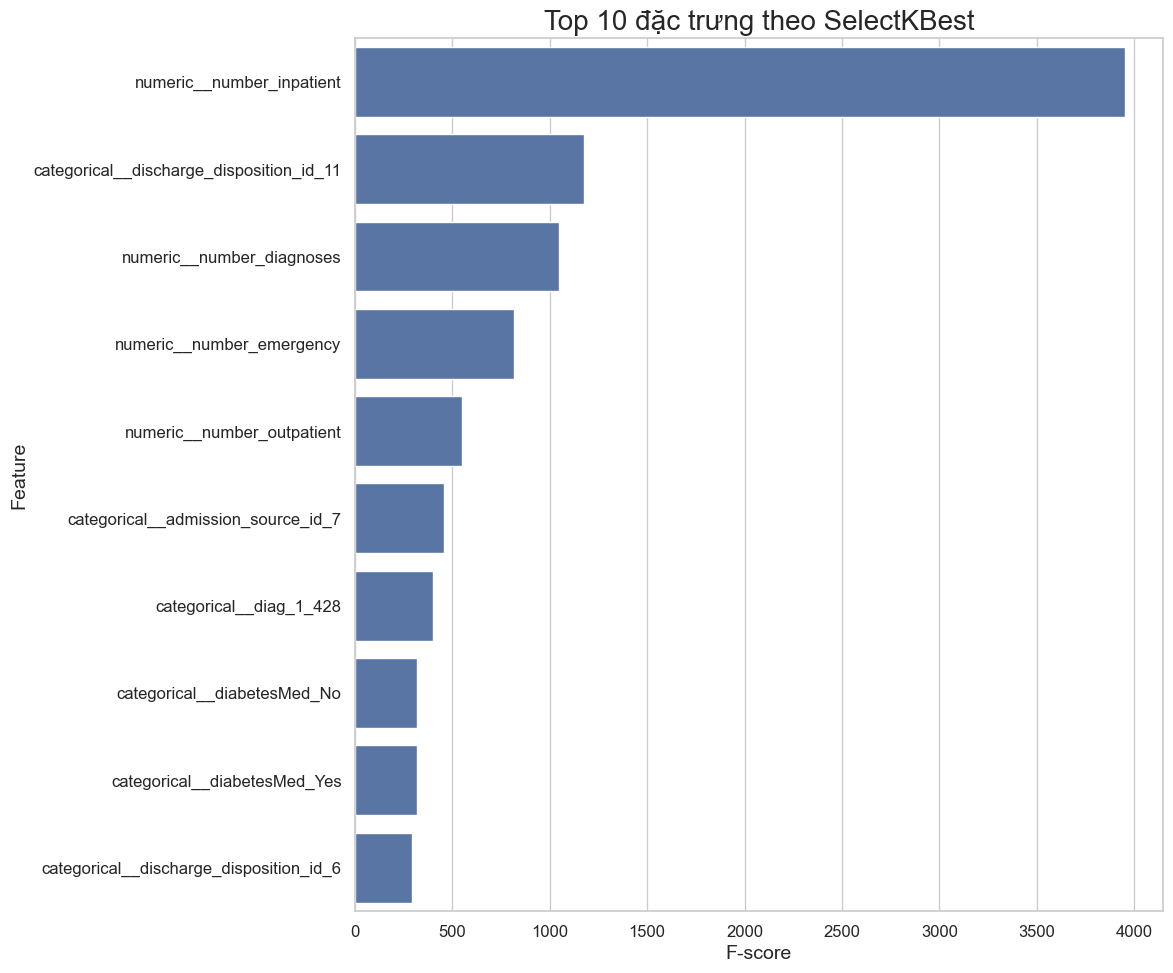
\includegraphics[width=0.8\textwidth]{../asset/top_10.png}
    \caption{Top 10 đặc trưng ảnh hưởng theo ANOVA}
\end{figure}

Xây dựng quy trình để Tiền xử lý cho loại dữ liệu dạng Numeric và Category. Đối với dữ liệu dạng số thực hiện xử lý các giá trị rỗng bằng giá trị trung vị, và dạng Category là tần suất xuất hiện nhiều nhất. Các model được lựa chọn để thử nghiệm là
Logistic Regression, Random Forest, XGBoost, LightGBM, và thực hiện một phép thử nhiều mô hình với Lazy Predict. 


\section*{Kết quả}
\begin{table}[H]
\centering
\caption{So sánh hiệu năng các mô hình học máy theo từng phương pháp đặc trưng}
\label{tab:model_performance}
\resizebox{\textwidth}{!}{
\begin{tabular}{|l|l|c|c|c|c|c|c|}
    \hline
    \textbf{Mô hình} & \textbf{Phương pháp} & \textbf{Accuracy} & \textbf{Balanced Acc.} & \textbf{Precision} & \textbf{Recall} & \textbf{F1} & \textbf{ROC-AUC} \\
    \hline
    \multirow{2}{*}{LightGBM} 
        & Base Model (All Features) & \textcolor{red}{0.653} & 0.646 & 0.630 & 0.569 & 0.598 & \textcolor{red}{0.709} \\
        & Selected Features  & 0.651 & 0.644 & 0.628 & 0.566 & 0.596 & 0.708 \\
    \hline
    \multirow{2}{*}{Logistic Regression} 
        & Base Model (All Features) & 0.637 & 0.636 & 0.596 & 0.620 & 0.608 & 0.695 \\
        & Selected Features  & 0.639 & 0.638 & 0.599 & 0.620 & 0.609 & 0.697 \\
    \hline
    \multirow{2}{*}{Random Forest} 
        & Base Model (All Features) & 0.641 & 0.640 & 0.598 & 0.634 & 0.615 & 0.698 \\
        & Selected Features  & 0.643 & \textcolor{red}{0.642} & 0.601 & \textcolor{red}{0.636} & \textcolor{red}{0.618} & 0.702 \\
    \hline
    \multirow{2}{*}{XGBoost} 
        & Base Model (All Features) & 0.652 & 0.642 & \textcolor{red}{0.637} & 0.541 & 0.585 & 0.707 \\
        & Selected Features  & 0.649 & 0.639 & 0.632 & 0.539 & 0.582 & 0.705 \\
    \hline
\end{tabular}
}
\end{table}

\begin{figure}[H]
    \centering
    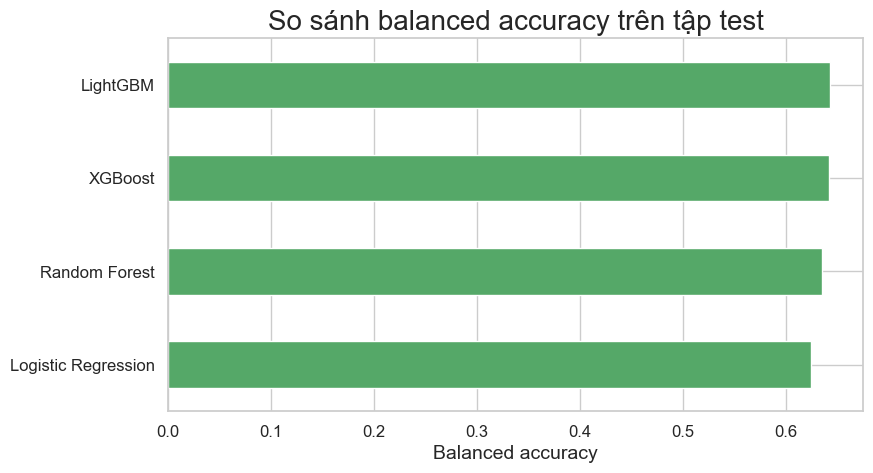
\includegraphics[width=0.8\textwidth]{../asset/balance_acc.png}\
    \caption{So sánh các mô hình dựa trên chỉ số Balance Accuracy}
\end{figure}

\begin{figure}[H]
    \centering
    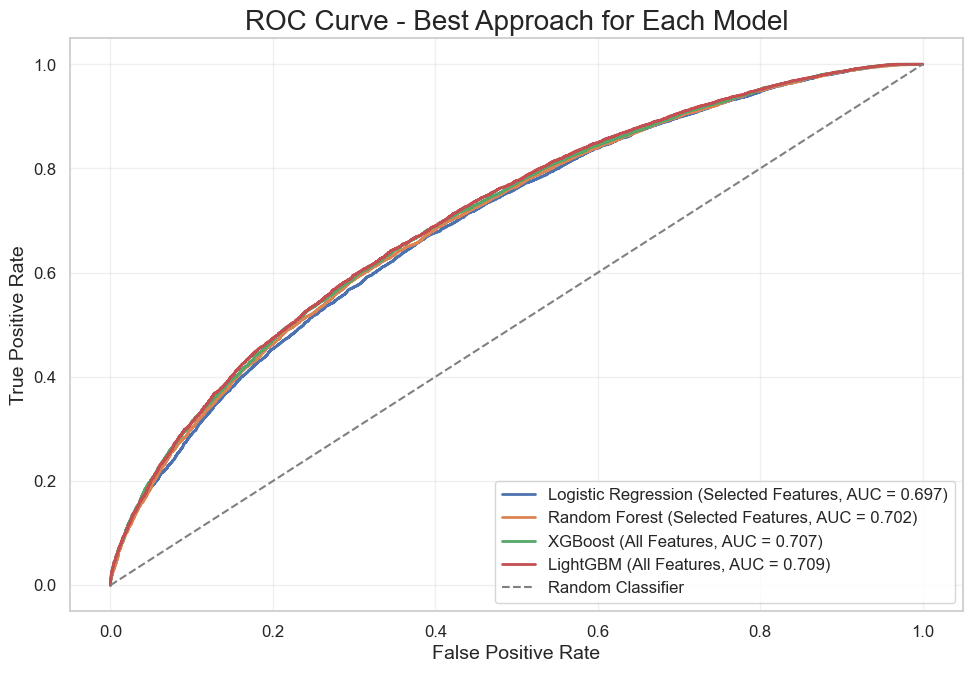
\includegraphics[width=0.95\textwidth]{../asset/ROC_AUC.png}\
    \caption{So sánh các mô hình dựa trên các chỉ số ROC và AUC}
\end{figure}

Vì thế việc lựa chọn mô hình đều tùy thuộc vào nhu cầu như khả năng chính xác cao hay tỉ lệ bỏ sót thấp.

\section*{Kết luận}
Từ kết quả trên, các mô hình học dữ liệu khá tốt và đối với các mô hình dạng cây như LightGBM, XGBoost sẽ học tốt hơn đặc biệt đạt hiệu năng cao trên "All Feature". Ngược lại, các mô hình hồi quy
với số lượng đặc trưng ít, khả năng học sẽ tốt hơn. Ngoài ra, trong quá trình phân tích cũng cho thấy độ tương quan giữa các thuộc tính rất nhiều, đặc biệt là các thuộc tính liên quan đến
xuất/nhập viên, chỉ số chuẩn đoán, và các chỉ số liên quan khác. Đặc biệt là đặc trưng xuất/nhập viện có ảnh hưởng rất lớn và từ đó cũng cho thấy được với một bệnh nhân hay xuất/nhập bệnh viện nhiều cũng đánh giá được một phần
sức khỏe của họ.

Từ những nghiên cứu trên, trong tương lai nếu bộ dữ liệu có cập nhật dữ liệu cho những năm gần đây thì sẽ phản ánh tốt hơn về tình trạng sức khỏe của người dân ở Mỹ cũng như tăng khả năng đánh giá, phân tích và ứng dụng các mô hình tiên tiến giúp cho các bệnh viện có được hiệu quả khai thác tốt hơn.
\end{document}